\documentclass[fr]{../../../../../../eplexam}
\usepackage{mathtools}
\usepackage{tikz}
\usepackage{enumitem}

\newcommand{\rang}{\mathrm{rang}}
\renewcommand{\Im}{\mathrm{Im}}

\allowdisplaybreaks

\usetikzlibrary{shapes,arrows,positioning,calc}
\tikzset{
	block/.style = {draw, fill=white, rectangle, minimum height=3em, minimum width=3em},
	sum/.style = {draw, fill=white, circle, node distance=1cm},
	input/.style = {coordinate},
	output/.style = {coordinate},
	pinstyle/.style = {pin edge={to-, thin, black}}
}

\hypertitle{Signaux et systèmes}{4}{FSAB}{1106}{2017}{Juin}
{Jean-Martin Vlaeminck}
{Luc Vandendorpe et Vincent Wertz}

\section{LV1}
Soit un système linéaire permanent (c-à-d invariant dans le temps) de réponse impulsionnelle $h(t)$ et de réponse en fréquence $H(j\omega)$.
On sait par ailleurs que le système est \emph{réel}.

On introduit $x(t) = \sin (\omega_0 t + \phi)$ dans ce système. Que vaut le signal qui est produit en sortie ? Démontrer le résultat.

\begin{solution}
On a
\[ x(t) = \sin (\omega_0 t + \phi) = \frac{e^{j(\omega_0 t + \phi)} - e^{-j(\omega_0 t + \phi)}}{2j} \]
et donc, la transformée de Fourier du signal est
\[ x(t) \leftrightarrow X(j\omega) = \frac{\pi}{j} e^{j\phi} \delta(\omega-\omega_0) - \frac{\pi}{j} e^{-j\phi} \delta(\omega+\omega_0)\]
Dès lors,
\begin{align*}
Y(j\omega) &= H(j\omega) \cdot X(j\omega) \\
&= H(j\omega) \cdot \left( \frac{\pi}{j} e^{j\phi} \delta(\omega - \omega_0) - \frac{\pi}{j} e^{-j\phi} \delta(\omega + \omega_0) \right) \\
&= H(j\omega_0) \frac{\pi}{j} e^{j\phi} \delta(\omega - \omega_0) - H(-j\omega_0) \frac{\pi}{j} e^{-j\phi} \delta(\omega + \omega_0) \\
&= \abs{H(j\omega_0)} \frac{\pi}{j} e^{j\phi} e^{j \arg(H(j\omega_0))} \delta(\omega-\omega_0) - \abs{H(-j\omega_0)} \frac{\pi}{j} e^{-j\phi} e^{j\arg( H(-j\omega_0))} \delta(\omega+\omega_0) \\
&= \abs{H(j\omega_0)} \frac{\pi}{j} e^{j\phi} e^{j \arg(H(j\omega_0))} \delta(\omega-\omega_0) - \abs{H(j\omega_0)} \frac{\pi}{j} e^{-j\phi} e^{-j\arg( H(j\omega_0))} \delta(\omega+\omega_0) \\
&= \abs{H(j\omega_0)} \left( \frac{\pi}{j} e^{j (\phi + \arg(H(j\omega_0)))} \delta(\omega-\omega_0) - \frac{\pi}{j} e^{-j(\phi + \arg(H(j\omega_0)))} \delta(\omega+\omega_0) \right)
\end{align*}
dont la transformée inverse est
\begin{align*}
Y(j\omega) \leftrightarrow y(t) &= \abs{H(j\omega_0)} \frac{e^{j (\omega_0 t + \phi + \arg(H(j\omega_0))} - e^{-j (\omega_0 t + \phi + \arg(H(j\omega_0)))}}{2j} \\
&= \abs{H(j\omega_0)} \sin (\omega_0 t + \phi + \arg(H(j\omega_0)))
\end{align*}
un résultat bien connu, et relativement logique : le signal de départ est déphasé de $\arg(H(j\omega_0))$, et est multiplié par $\abs{H(j\omega_0)}$.

Rappelons que, pour un système réel, la partie réelle de la fonction de transfert est paire et la partie imaginaire est impaire, ce qui a pour conséquence que le module est pair et l'argument est impair.
\end{solution}

\section{LV2}
On s'intéresse à la transformée de Fourier discrète (TFD) d'un vecteur $X$ de taille $N = 8$ comprenant les échantillons d'un signal $x[n]$ \emph{réel}, pour $n = 0, \dots, N-1$.

La TFD produit un vecteur $X = [X[0], \dots, X[N-1]]^T$
\begin{enumerate}[label=(\alph*)]
	\item Sachant que la période d'échantillonnage du signal temporel est $T$, quelles sont les positions des échantillons $X[k]$ (en fréquences vraies, c-à-d en hertz) ? Justifier.
	\item Sachant que le signal $x[n]$ de départ est réel, quelles sont les propriétés ou liens dont bénéficient les coefficients $X[k]$ des produits ?
	\item On définit le signal $y[n] = (-1)^n x[n]$. Que vaut la DFT $Y[k]$ de $y[n]$, en fonction de $X[k]$ ?
\end{enumerate}

\begin{solution}
\begin{enumerate}[label=(\alph*)]
	\item C'est probablement la question qui requiert le plus d'avoir une bonne vue d'ensemble de toutes les transformées. Pour déterminer ces \og fréquences vraies\fg{}, ainsi que ce qu'elles représentent, il faut se rappeler des relations entre la DFT et la DTFT, et entre la DTFT de l'échantillonnage d'un signal, la FT originale et la FT de l'échantillonnage.
	\begin{itemize}
		\item La transformée de Fourier discrète d'un signal $a[n]$, de durée finie $N$, (TFD, ou DFT en anglais) peut s'interpréter comme l'échantillonnage de la DTFT (transformée de Fourier en temps discret) de ce signal $a[n]$. En notant $a_P[n]$ le signal obtenu en inversant la DFT\footnote{Au facteur $N$ près, c'est la même expression que pour la série de Fourier.}, cet échantillonnage a comme conséquence de rendre le signal $a_P[n]$ périodique, de période $N$. Comme il y a $N$ échantillons sur une période de $2\pi$, on écrit $A[k] = X\left(e^{j \frac{2k\pi}{N}}\right)$, avec donc des échantillons espacés de $\frac{2\pi}{N}$ dans la fréquence $\Omega$.
		\item Étant donné un signal $a(t)$, son échantillonnage $a_e(t)$ et $a_e[n]$ à la période d'échantillonnage $T$ donne une transformée de Fourier $A_e(j\omega)$ périodique de période $\frac{2\pi}{T}$, qui est une mise à l'échelle de la transformée de Fourier en temps discrète $A_e(e^{j\Omega})$, de période $2\pi$. Les fréquences $\omega$ et $\Omega$ sont reliées par la relation $\omega = \Omega/T$.
		\item Enfin, la transformée de Fourier $A(j\omega)$, utilisant des fréquences en radians par seconde, peut être convertie en une transformée de Fourier $A(jf)$ utilisant des hertz via $\omega=2\pi f$.
	\end{itemize}
	En mettant tout cela ensemble, on obtient que la position, en hertz, de $X[k]$ va être :
	\[ k \leftrightarrow \Omega = \frac{2k\pi}{N} \leftrightarrow \omega = \frac{2k\pi}{N T} \leftrightarrow f = \frac{k}{N T} \]
	Et donc, chaque $X[k]$, échantillon de la DTFT, correspond à la valeur de la transformée du signal échantillonné à une fréquence de $\frac{k}{NT}$.

	\item La partie réelle des coefficients $X[k]$ est un signal pair, et la partie imaginaire est un signal impair. On dit que le signal a la propriété de \emph{symétrie conjuguée} (\emph{complex-conjugate symmetric}) : $X[-k] = X[k]^*$, où $a*$ dénote le complexe conjugué de $a$. La démonstration est à la section 3.9.1 de~\cite{haykinvanveen}, page 256.

	Une autre propriété sympathique est que $\Im(X[mN]) = 0$ : la DFT est purement réel à chaque multiple de $N$.

	% TODO compléter par d'autres propriétés, s'il y en a.

	\item En reprenant la définition, et en se souvenant que $N = 8$ est pair,
	\begin{align*}
	Y[k] &= \sum_{n=0}^{N-1} y[n] e^{- \frac{2 \pi j k n}{N}} \\
	&= \sum_{n=0}^{N-1} x[n] (-1)^n e^{- \frac{2 \pi j k n}{N}} \\
	&= \sum_{n=0}^{N-1} x[n] e^{- \pi j n} e^{- \frac{2 \pi j k n}{N}} \\
	&= \sum_{n=0}^{N-1} x[n] e^{- \frac{2 \pi j k n + \pi j N n}{N}} \\
	&= \sum_{n=0}^{N-1} x[n] e^{- \frac{2 \pi j (k + \frac{N}{2}) n}{N}} \\
	&= X \left[ k + \frac{N}{2} \right]
	\end{align*}
	On a simplement décalé la DFT de $N/2$.

	Une autre démonstration, basée sur le produit des signaux $x[n]$ et $h[n]=(-1)^n$ en temporel, et donc la convolution des signaux en fréquentiels :
	% Version cosinus :
%	\begin{align*}
%	h[n] &= (-1)^n \\
%	&= \cos(pi n) \\
%	&= \cos\left(\frac{2\pi}{N} \cdot \frac{N}{2} n\right)
%	\end{align*}
%	\begin{align*}
%	\longleftrightarrow H[k] &= \frac{N}{2} \quad k = \frac{N}{2} + mN, m\in \mathbf{Z}
%	&\quad + \frac{N}{2} \quad k = -\frac{N}{2} + mN, m\in \mathbf{Z} \\
%	&= 2\cdot\frac{N}{2} \quad k=\frac{(2m+1)N}{2}, m\in\mathbf{Z} \\
%	&= \begin{cases}
%	N & \text{si} k=\frac{(2m+1)N}{2}, m\in\mathbf{Z} \\
%	0 & \text{sinon}
%	\end{cases}
%	\end{align*}
	% Version fondamentale :
	\begin{align*}
	h[n]=(-1)^n \longleftrightarrow H[k] &= \sum_{n=0}^{N-1} h[n] e^{-\frac{2\pi j k n}{N}}
	= \sum_{n=0}^{N-1} e^{-j \pi n} e^{-\frac{j 2 \pi k n}{N}}
	= \sum_{n=0}^{N-1} e^{-j \pi \frac{N + 2k}{N} n} \\
	&= \frac{1 - e^{-j \pi (N+2k)}}{1 - e^{-j\pi \frac{N+2k}{N}}}
	\end{align*}
	Le numérateur s'annule pour tout $k$, $N$ étant pair. La transformée ne pouvant pas être nulle, on regarde à quelles conditions le dénominateur s'annule, en espérant que ça sauve notre transformée. Le dénominateur s'annule quand
	\begin{align*}
	e^{-j\pi\frac{N+2k}{N}} = 1 \Leftrightarrow
	\pi\frac{N+2k}{N} &= 2m\pi \quad m\in\mathbf{Z} \\
	N+2k &= 2mN \\
	k &= (2m-1)\frac{N}{2}
	\end{align*}
	autrement dit, lorsque $k=\frac{N}{2}, \frac{3N}{2}, \dots$. Dans ces cas, on a
	\begin{equation*}
	H\left[\frac{N}{2}\right] = \sum_{n=0}^{N-1} (-1)^n e^{-\frac{2 \pi j N n}{2 N}}
	= \sum_{n=0}^{N-1} (-1)^n e^{- \pi j n}
	= \sum_{n=0}^{N-1} (-1)^n (-1)^n
	= \sum_{n=0}^{N-1} 1^n = N
	\end{equation*}
	ce qui donne finalement
	\[ H[k] = \begin{cases}
	N & \text{ si } k=\frac{(2m+1) N}{2}, m\in \mathbf{Z} \\
	0 & \text{ sinon} \\
	\end{cases} \]
	On peut maintenant écrire $Y[k]$, en convoluant les deux transformées :
	\begin{align*}
	Y[k] = \frac{1}{N} X[k] \circledast H[k]
	= \frac{1}{N} \sum_{l=0}^{N-1} H[l] X[k-l]
	\end{align*}
	Comme $H[l]=0$ partout sauf en $N/2$, où il vaut $N$:
	\[ Y[k] = X\left[k-\frac{N}{2}\right] = X\left[k+\frac{N}{2}\right] \quad \text{par périodicité} \]
	soit le même résultat qu'avant.
\end{enumerate}
\end{solution}

\section{LV3}
On génère un signal périodique $x(t) = \sin (2 \pi f_0 t)$. Ce signal est d'abord échantillonné par un échantillonneur\footnote{Sans blague ?} qui fonctionne à la fréquence $f_e$. Ensuite, le résultat de l'échantillonnage est interpolé par un filtre réel, fonctionnant en temps continu de type passe-bas idéal et de fréquence de coupure $f_e/2$ (il laisse donc passer toutes les fréquences $f$ telles que $\abs{f} \le f_e/2$).%FIXME < ou <= ?
Le schéma complet est décrit ci-dessous.
\begin{center}
	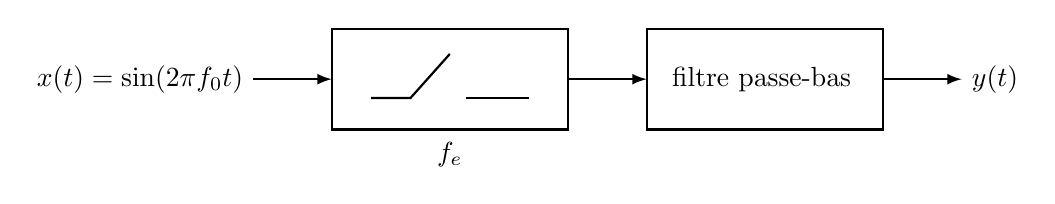
\begin{tikzpicture}[y=0.8cm]
	\draw (0, 0) node[left] {$x(t) = \sin (2 \pi f_0 t)$};
	\draw[thick, ->, >=latex] (0, 0) -- (1, 0);
	\draw[thick] (1, -0.8) rectangle (4, 0.8);
	\draw[thick] (1.5, -0.3) -- (2, -0.3) -- (2.5, 0.4);
	\draw[thick] (2.7, -0.3) -- (3.5, -0.3);
	\draw (2.5, -1.2) node[] {$f_e$};
	\draw[thick, ->, >=latex] (4, 0) -- (5, 0);
	\draw[thick] (5, -0.8) rectangle (8, 0.8);
	\draw (5.2, 0) node[right] {filtre passe-bas};
	\draw[thick, ->, >=latex] (8, 0) -- (9, 0) node[right] {$y(t)$};
	\end{tikzpicture}
\end{center}
\begin{enumerate}[label=(\alph*)]
	\item Représentez graphiquement le spectre du signal obtenu en sortie du filtre analogique lorsque $f_0 = f_e/4$. Justifiez.
	\item Pareil lorsque $f_0 = 7f_e/8$. Justifiez.
	\item Représentez graphiquement le spectre du signal obtenu en sortie du filtre analogique lorsque, à $f_e$ fixé, on augmente $f_0$ de $0$ jusque $3f_e/2$. Justifiez.
\end{enumerate}

\begin{solution}
L'échantillonnage va provoquer une réplication, tous les $f_e$ (ou $\omega_e = 2 \pi f_e$), du spectre du signal de départ. Le filtre passe-bas va ensuite éliminer l'ensemble de ce spectre qui se trouve en dehors de l'intervalle $[-f_e/2, f_e/2]$ ; cela va éliminer une partie des réplicants, mais va peut-être aussi éliminer une partie du spectre du signal de départ, ou va laisser des réplicants.

Sur l'ensemble des figures qui suivent, le spectre du signal en sortie de l'échantillonneur est indiqué en traitillés verts, et le spectre du signal en sortie du filtre passe-bas est indiqué en traits continus verts.
Le spectre original (transformée de Fourier appliquée à un signal périodique) est indiqué par des traits bleus, ainsi que sur la figure ci-dessous.
Enfin, la zone grise indique l'ensemble des fréquences qui sont acceptées par le filtre passe-bas.

Celui-ci est d'ailleurs
\[ X(j\omega) = \frac{\pi}{j} \delta(\omega - 2\pi f_0) - \frac{\pi}{j} \delta(\omega + 2 \pi f_0) \]
et chacun des spectres resteront d'ailleurs purement imaginaires, sans partie réelle, qui ne sera donc pas représentée.

Lors de l'examen, seul le spectre en sortie du filtre passe-bas était demandé ; les autres spectres ne devaient pas être dessinés. Également, le spectre était demandé, pas son module, ce qui explique le signe des impulsions de la figure suivante\footnote{Remarquez que la graduation sur l'axe est de $\pi/j$ : le pic de gauche a en fait une partie imaginaire positive.}.
\begin{center}
\begin{tikzpicture}
\draw[thick, ->, >=latex] (-3, 0) -- (3, 0) node[below right] {$f$};
\draw[thick, ->, >=latex] (0, -1.6) -- (0, 2) node[above right] {$X(jf)$};
\draw[thick, Green, ->, >=stealth] (1, 0) -- (1, 1.5);
\draw (1, 0) node[below] {$f_0$};
\draw[thick, Green, ->, >=stealth] (-1, 0) -- (-1, -1.5);
\draw (-1, 0) node[above] {$-f_0$};
\draw (0.1, 1.5) -- (-0.1, 1.5) node[left] {$\frac{\pi}{j}$};
\end{tikzpicture}
\end{center}

\begin{enumerate}[label=(\alph*)]
	\item Lorsque $f_0 = f_e/4$, l'hypothèse du théorème d'échantillonnage est satisfaite (la fréquence d'échantillonnage $f_e$ est strictement supérieure au double de la fréquence $f_0$), et donc le signal de départ peut être reconstruit à partir du signal en sortie du filtre passe-bas ; il n'y a pas de repli spectral.
	\begin{center}
	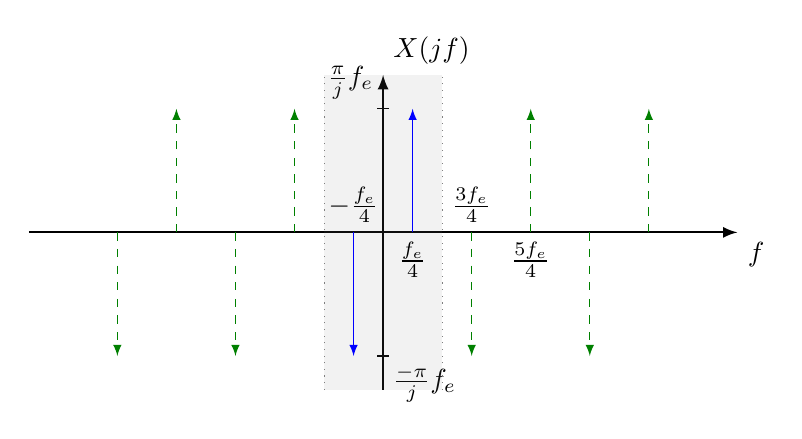
\begin{tikzpicture}[x=1.5cm, y=0.5cm]
	% Une unité TikZ horizontale = un multiple de f_e (fréquence d'échantillonnage, 2*limites du filtre passe-bas)
	% Une unité TikZ verticale = un multiple de f_e (fréquence d'échantillonnage, le facteur par lequel est multiplié chacune des répliques du signal périodique quand on l'échantillonne).
	% Axes
	\draw[thick, ->, >=latex] (-3, 0) -- (3, 0) node[below right] {$f$};
	\draw[thick, ->, >=latex] (0, -4) -- (0, 4) node[above right] {$X(jf)$};
	\draw (0.05, 3.14) -- (-0.05, 3.14) (0, 3.14) node[above left] {$\frac{\pi}{j}f_e$};
	\draw (-0.05, -3.14) -- (0.05, -3.14) (0, -3.14) node[below right] {$\frac{-\pi}{j}f_e$};
	% Zone du filtre
	\draw[thin, dotted, Gray] (-0.5, -4) -- (-0.5, 4);
	\draw[thin, dotted, Gray] (0.5, -4) -- (0.5, 4);
	\fill[gray, opacity=0.1] (-0.5, -4) rectangle (0.5, 4);
	%\draw (-0.5, 0) node[below left] {$-\frac{f_e}{2}$};
	%\draw (0.5, 0) node[above right] {$\frac{f_e}{2}$};
	% Impulsions, groupées par réplique.
	\draw[thin, Green, dashed, -latex] (-2.25, 0) -- (-2.25, -3.14);
	\draw[thin, Green, dashed, -latex] (-1.75, 0) -- (-1.75, 3.14);
	\draw[thin, Green, dashed, -latex] (-1.25, 0) -- (-1.25, -3.14);
	\draw[thin, Green, dashed, -latex] (-0.75, 0) -- (-0.75, 3.14);
	\draw[thin, blue, -latex] (-0.25, 0) -- (-0.25, -3.14);
	\draw[thin, blue, -latex] (0.25, 0) -- (0.25, 3.14);
	\draw[thin, Green, dashed, -latex] (0.75, 0) -- (0.75, -3.14);
	\draw[thin, Green, dashed, -latex] (1.25, 0) -- (1.25, 3.14);
	\draw[thin, Green, dashed, -latex] (1.75, 0) -- (1.75, -3.14);
	\draw[thin, Green, dashed, -latex] (2.25, 0) -- (2.25, 3.14);
	% Coordonnées
	\draw (-0.25, 0) node[above] {$-\frac{f_e}{4}$};
	\draw (0.25, 0) node[below] {$\frac{f_e}{4}$};
	\draw (0.75, 0) node[above] {$\frac{3f_e}{4}$};
	\draw (1.25, 0) node[below] {$\frac{5f_e}{4}$};
	\end{tikzpicture}
	\end{center}
	\item Cette fois, l'hypothèse du théorème de Shannon n'est plus satisfaite, et il y a repli spectral (\emph{aliasing}) ; après le filtre passe-bas, il est impossible de reconstituer le signal de départ. En fait, le signal s'est transformé\footnote{Il a pris une autre forme, une sorte d'alias.} en $y(t) = -\sin (2 \pi f_e / 8)$.
	\begin{center}
	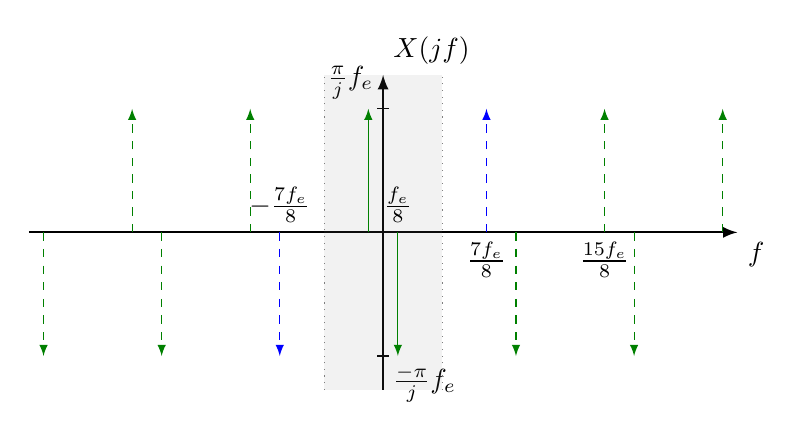
\begin{tikzpicture}[x=1.5cm, y=0.5cm]
	% Axes
	\draw[thick, ->, >=latex] (-3, 0) -- (3, 0) node[below right] {$f$};
	\draw[thick, ->, >=latex] (0, -4) -- (0, 4) node[above right] {$X(jf)$};
	\draw (0.05, 3.14) -- (-0.05, 3.14) (0, 3.14) node[above left] {$\frac{\pi}{j}f_e$};
	\draw (-0.05, -3.14) -- (0.05, -3.14) (0, -3.14) node[below right] {$\frac{-\pi}{j}f_e$};
	% Zone du filtre
	\draw[thin, dotted, Gray] (-0.5, -4) -- (-0.5, 4);
	\draw[thin, dotted, Gray] (0.5, -4) -- (0.5, 4);
	\fill[gray, opacity=0.1] (-0.5, -4) rectangle (0.5, 4);
	%\draw (-0.5, 0) node[below left] {$-\frac{f_e}{2}$};
	%\draw (0.5, 0) node[above right] {$\frac{f_e}{2}$};
	% Impulsions, groupées par réplique.
	\draw[thin, Green, dashed, -latex] (-2.125, 0) -- (-2.125, 3.14);
	\draw[thin, Green, dashed, -latex] (-2.875, 0) -- (-2.875, -3.14);
	\draw[thin, Green, dashed, -latex] (-1.125, 0) -- (-1.125, 3.14);
	\draw[thin, Green, dashed, -latex] (-1.875, 0) -- (-1.875, -3.14);
	\draw[thin, Green, -latex] (-0.125, 0) -- (-0.125, 3.14);
	\draw[thin, dashed, blue, -latex] (-0.875, 0) -- (-0.875, -3.14);
	\draw[thin, dashed, blue, -latex] (0.875, 0) -- (0.875, 3.14);
	\draw[thin, Green, -latex] (0.125, 0) -- (0.125, -3.14);
	\draw[thin, Green, dashed, -latex] (1.875, 0) -- (1.875, 3.14);
	\draw[thin, Green, dashed, -latex] (1.125, 0) -- (1.125, -3.14);
	\draw[thin, Green, dashed, -latex] (2.875, 0) -- (2.875, 3.14);
	\draw[thin, Green, dashed, -latex] (2.125, 0) -- (2.125, -3.14);
	% Coordonnées
	\draw (-0.875, 0) node[above] {$-\frac{7f_e}{8}$};
	\draw (0.875, 0) node[below] {$\frac{7f_e}{8}$};
	\draw (0.125, 0) node[above] {$\frac{f_e}{8}$};
	\draw (1.875, 0) node[below] {$\frac{15f_e}{8}$};
	\end{tikzpicture}
	\end{center}
	\item Pour $0 < f_0 < f_e/2$, le spectre du signal $x(t)$ ne subit aucun repli spectral, et ressort indemne du filtre passe-bas.
	% TODO insérer figure
	\begin{center}
	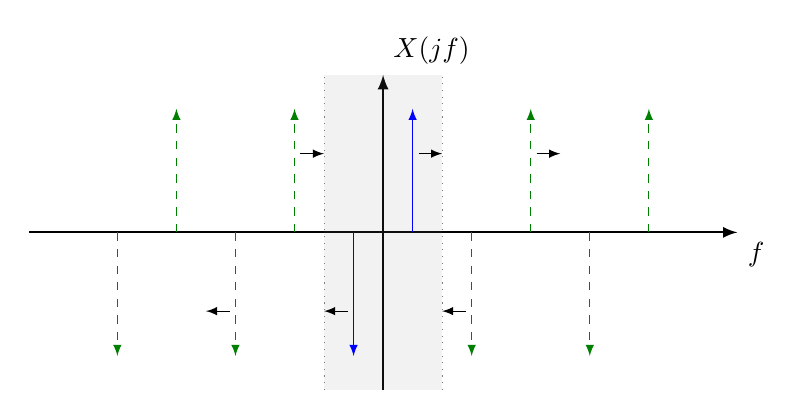
\begin{tikzpicture}[x=1.5cm, y=0.5cm]
	% Axes
	\draw[thick, ->, >=latex] (-3, 0) -- (3, 0) node[below right] {$f$};
	\draw[thick, ->, >=latex] (0, -4) -- (0, 4) node[above right] {$X(jf)$};
	% Zone du filtre
	\draw[thin, dotted, Gray] (-0.5, -4) -- (-0.5, 4);
	\draw[thin, dotted, Gray] (0.5, -4) -- (0.5, 4);
	\fill[gray, opacity=0.1] (-0.5, -4) rectangle (0.5, 4);
	%\draw (-0.5, 0) node[below left] {$-\frac{f_e}{2}$};
	%\draw (0.5, 0) node[above right] {$\frac{f_e}{2}$};
	% Impulsions, groupées par réplique.
	\draw[thin, Green, dashed, -latex] (-2.25, 0) -- (-2.25, -3.14);
	\draw[thin, Green, dashed, -latex] (-1.75, 0) -- (-1.75, 3.14);

	\draw[thin, Green, dashed, -latex] (-1.25, 0) -- (-1.25, -3.14);
	\draw[thin, -latex] (-1.3, -2) -- (-1.5, -2);
	\draw[thin, Green, dashed, -latex] (-0.75, 0) -- (-0.75, 3.14);
	\draw[thin, -latex] (-0.7, 2) -- (-0.5, 2);

	\draw[thin, blue, -latex] (-0.25, 0) -- (-0.25, -3.14);
	\draw[thin, -latex] (-0.3, -2) -- (-0.5, -2);
	\draw[thin, blue, -latex] (0.25, 0) -- (0.25, 3.14);
	\draw[thin, -latex] (0.3, 2) -- (0.5, 2);

	\draw[thin, Green, dashed, -latex] (0.75, 0) -- (0.75, -3.14);
	\draw[thin, -latex] (0.7, -2) -- (0.5, -2);
	\draw[thin, Green, dashed, -latex] (1.25, 0) -- (1.25, 3.14);
	\draw[thin, -latex] (1.3, 2) -- (1.5, 2);

	\draw[thin, Green, dashed, -latex] (1.75, 0) -- (1.75, -3.14);
	\draw[thin, Green, dashed, -latex] (2.25, 0) -- (2.25, 3.14);
	\end{tikzpicture}
	\end{center}

	Pour $f_0 = f_e/2$, les deltas se superposent parfaitement, et s'annulent ; le spectre du signal disparait en sortie de l'échantillonneur (ce qui est logique, le signal étant nul à chaque échantillon), et donc le signal en sortie du filtre passe-bas est nul.

	Pour $f_e/2 < f_0 < f_e$, il y a repli spectral, le spectre du signal original sortant de la fenêtre du filtre passe-bas, et les diracs des répliques adjacentes entrant dans la fenêtre. Le signal en sortie du filtre passe-bas n'est plus le même que le signal de départ, et la fréquence de ce signal diminue (les diracs sortant du filtre se rapprochent de $0$).\footnote{En notant $f_1$ la fréquence de ce signal, on peut en fait constater que $f_1 = f_e - f_0$.}
	% TODO insérer figure
	\begin{center}
	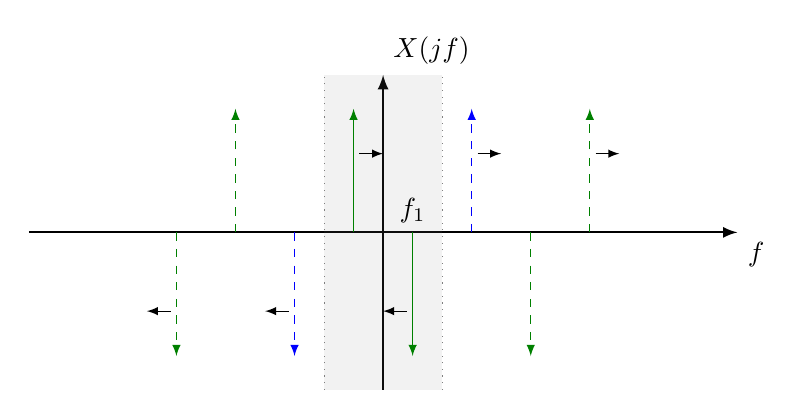
\begin{tikzpicture}[x=1.5cm, y=0.5cm]
	% Axes
	\draw[thick, ->, >=latex] (-3, 0) -- (3, 0) node[below right] {$f$};
	\draw[thick, ->, >=latex] (0, -4) -- (0, 4) node[above right] {$X(jf)$};
	% Zone du filtre
	\draw[thin, dotted, Gray] (-0.5, -4) -- (-0.5, 4);
	\draw[thin, dotted, Gray] (0.5, -4) -- (0.5, 4);
	\fill[gray, opacity=0.1] (-0.5, -4) rectangle (0.5, 4);
	%\draw (-0.5, 0) node[below left] {$-\frac{f_e}{2}$};
	%\draw (0.5, 0) node[above right] {$\frac{f_e}{2}$};
	% Impulsions, groupées par réplique.
	\draw[thin, Green, dashed, -latex] (-1.25, 0) -- (-1.25, 3.14);

	\draw[thin, Green, dashed, -latex] (-1.75, 0) -- (-1.75, -3.14);
	\draw[thin, -latex] (-1.8, -2) -- (-2, -2);
	\draw[thin, Green, -latex] (-0.25, 0) -- (-0.25, 3.14);
	\draw[thin, -latex] (-0.2, 2) -- (0, 2);

	\draw[thin, dashed, blue, -latex] (-0.75, 0) -- (-0.75, -3.14);
	\draw[thin, -latex] (-0.8, -2) -- (-1, -2);
	\draw[thin, dashed, blue, -latex] (0.75, 0) -- (0.75, 3.14);
	\draw[thin, -latex] (0.8, 2) -- (1, 2);

	\draw[thin, Green, -latex] (0.25, 0) -- (0.25, -3.14);
	\draw (0.25, 0) node[above] {$f_1$};
	\draw[thin, -latex] (0.2, -2) -- (0, -2);
	\draw[thin, Green, dashed, -latex] (1.75, 0) -- (1.75, 3.14);
	\draw[thin, -latex] (1.8, 2) -- (2, 2);

	\draw[thin, Green, dashed, -latex] (1.25, 0) -- (1.25, -3.14);
	\end{tikzpicture}
	\end{center}

	Pour $f_0 = f_e$, le signal ressortant de l'échantillonneur est de nouveau nul, pour les mêmes raisons que $f_0 = f_e/2$.

	Pour $f_e < f_0 < 3f_e/2$, il y a toujours repli spectral, mais les diracs des répliques s'éloignent de $0$, et la fréquence du signal de sortie\footnote{Égal à $f_2 = f_0 - f_e$.} augmente.
	% TODO insérer figure
	\begin{center}
	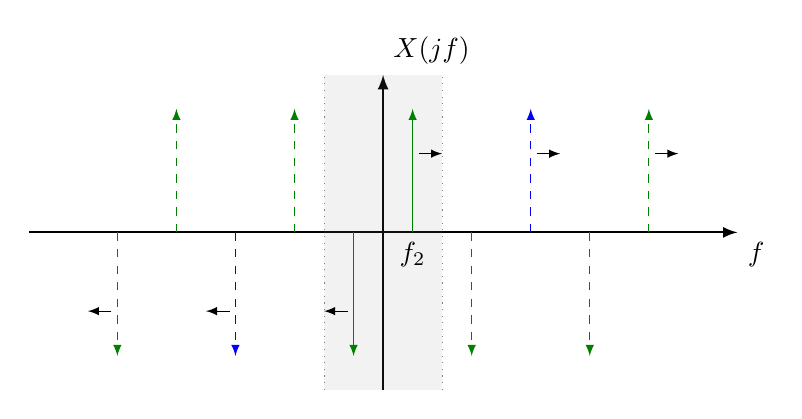
\begin{tikzpicture}[x=1.5cm, y=0.5cm]
	% Axes
	\draw[thick, ->, >=latex] (-3, 0) -- (3, 0) node[below right] {$f$};
	\draw[thick, ->, >=latex] (0, -4) -- (0, 4) node[above right] {$X(jf)$};
	% Zone du filtre
	\draw[thin, dotted, Gray] (-0.5, -4) -- (-0.5, 4);
	\draw[thin, dotted, Gray] (0.5, -4) -- (0.5, 4);
	\fill[gray, opacity=0.1] (-0.5, -4) rectangle (0.5, 4);
	%\draw (-0.5, 0) node[below left] {$-\frac{f_e}{2}$};
	%\draw (0.5, 0) node[above right] {$\frac{f_e}{2}$};
	% Impulsions, groupées par réplique.
	\draw[thin, Green, dashed, -latex] (-1.75, 0) -- (-1.75, 3.14);
	\draw[thin, Green, dashed, -latex] (-0.75, 0) -- (-0.75, 3.14);

	\draw[thin, Green, dashed, -latex] (-2.25, 0) -- (-2.25, -3.14);
	\draw[thin, -latex] (-2.3, -2) -- (-2.5, -2);
	\draw[thin, Green, -latex] (0.25, 0) -- (0.25, 3.14);
	\draw[thin, -latex] (0.3, 2) -- (0.5, 2);
	\draw (0.25, 0) node[below] {$f_2$};

	\draw[thin, dashed, blue, -latex] (-1.25, 0) -- (-1.25, -3.14);
	\draw[thin, -latex] (-1.3, -2) -- (-1.5, -2);
	\draw[thin, dashed, blue, -latex] (1.25, 0) -- (1.25, 3.14);
	\draw[thin, -latex] (1.3, 2) -- (1.5, 2);

	\draw[thin, Green, -latex] (-0.25, 0) -- (-0.25, -3.14);
	\draw[thin, -latex] (-0.3, -2) -- (-0.5, -2);
	\draw[thin, Green, dashed, -latex] (2.25, 0) -- (2.25, 3.14);
	\draw[thin, -latex] (2.3, 2) -- (2.5, 2);

	\draw[thin, Green, dashed, -latex] (0.75, 0) -- (0.75, -3.14);
	\draw[thin, Green, dashed, -latex] (1.75, 0) -- (1.75, -3.14);
	\end{tikzpicture}
	\end{center}
\end{enumerate}
\end{solution}

\section{VW1}
On considère un système causal décrit par la fonction de transfert
\[G(s) = \frac{s+1}{(s-1)(s^2 + \frac{3}{2} s + 1)}\]

\begin{enumerate}[label=(\alph*)]
	\item Ce système est-il stable EBSB ?
	\item Est-il possible de concevoir un système de fonctions de transfert $H(s)$ dont le degré du numérateur est inférieur au degré du dénominateur et tel que la connexion en série représentée ci-dessous soit stable ?
	\begin{center}
		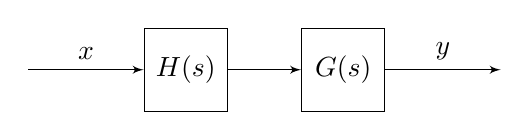
\begin{tikzpicture}[auto, node distance=2cm, >=latex']
		\node [input, name=input] {$x$};
		\node [block, right of=input] (htf) {$H(s)$};
		\node [block, right of=htf] (gtf) {$G(s)$};
		\node [output, right of=gtf] (output) {$y$};
		\draw [->] (input) -- node {$x$} (htf);
		\draw [->] (htf) -- (gtf);
		\draw [->] (gtf) -- node[name=y] {$y$} (output);
		\end{tikzpicture}
	\end{center}
	\item Proposer un tel système.
	\item Est-il possible de trouver un gain $K$ tel que le feedback représenté à la figure suivante donne lieu à une fonction de transfert stable ? Quelles sont les éventuelles conditions sur $K$ ?
	\begin{center}
		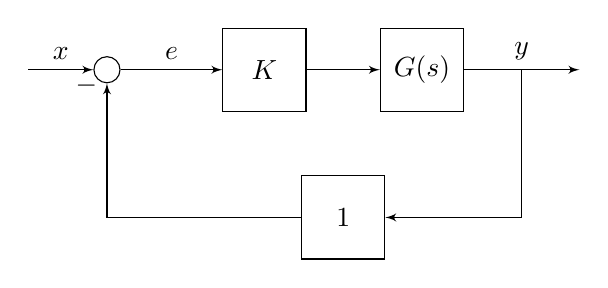
\begin{tikzpicture}[auto, node distance=2cm, >=latex']
			\node [input, name=input] {$x$};
			\node [sum, right of=input] (sum) {};
			\node [block, right of=sum] (factor) {$K$};
			\node [block, right of=factor] (tf) {$G(s)$};
			\node [output, right of=tf] (output) {$y$};
			\draw [->] (factor) -- node[name=u] {} (tf);
			\node [block, below of=u] (one) {$1$};
			\draw [->] (input) -- node {$x$} (sum);
			\draw [->] (sum) -- node {$e$} (factor);
			\draw [->] (tf) -- node[name=y] {$y$} (output);
			\draw [->] (y) |- (one);
			\draw [->] (one) -| node[pos=0.99] {$-$} (sum);
		\end{tikzpicture}
	\end{center}
	\item Si le but est de stabiliser la fonction de transfert, quel schéma semble préférable et pourquoi ?
\end{enumerate}

\begin{solution}
\begin{enumerate}[label=(\alph*)]
	\item Les pôles de la fonction de transfert sont en $1$, en $-\frac{3}{4} + j\frac{\sqrt{7}}{4}$ et en $-\frac{3}{4} - j\frac{\sqrt{7}}{4}$. Comme $1$ est à droite de l'axe imaginaire, et que le système est causal, le système n'est pas stable BIBO (il faudrait que tous les pôles soient à gauche de l'axe imaginaire, donc à partie réelle négative).
	\item Pour cela, il faut une fonction de transfert dont le numérateur élimine le pôle à partie réelle positive, et dont les pôles soient à partie réelle négative. Par exemple,
	\[H(s) = \frac{s-1}{(s+1)(s+2)}\]
	%FIXME pas sûr
	\item La fonction de transfert du système complet s'obtient en écrivant que
	\[ Y(s) = K G(s) (X(s)-Y(s)) \]
	ce qui donne
	\[ \frac{Y(s)}{X(s)} = \frac{K G(s)}{1+K G(s)} \]
	soit
	\begin{align*}
	\frac{Y(s)}{X(s)} &= \frac{K \frac{s+1}{(s-1) \left(s^2 + \frac{3}{2}s + 1\right)}}{1+K \frac{s+1}{(s-1)\left(s^2 + \frac{3}{2}s + 1\right)}} \\
	&= \frac{K (s+1)}{s^3 + \frac{1}{2}s^2 - \frac{1}{2}s - 1 + Ks + K}
	\end{align*}
	Pour que la fonction de transfert soit stable, il faut donc s'assurer que le dénominateur ne contienne pas de racines à partie réelle positive. Pour cela, on utilise le critère de Routh-Hurwitz sur le polynôme $s^3 + \frac{1}{2} s^2 + (K - \frac{1}{2}) s + (K-1)$ :

	\begin{center}
	\begin{tabular}{ccc}
	$1$ & $K-\frac{1}{2}$ & \dots \\
	$\frac{1}{2}$ & $K-1$ & \dots \\
	$K - \frac{1}{2} - \frac{K-1}{\frac{1}{2}} = -K +\frac{3}{2}$ & 0 & \dots \\
	$K - 1$ & 0 & \dots \\
	0 & 0 & \dots
	\end{tabular}
	\end{center}

	Le critère de Routh-Hurwitz stipule que le nombre de racines à partie réelle positive est égal au nombre de changement de signe des nombres de la première colonne. Comme on veut déterminer l'ensemble des $K$ tels que toutes les racines ont des parties réelles négatives, il faut que tous les nombres de la première colonne soient strictement positifs, et donc il faut que
	\[
	\begin{cases}
	\frac{3}{2} - K > 0 \Rightarrow K < \frac{3}{2} \\
	K - 1 > 0 \Rightarrow K > 1 \\
	\end{cases}
	\]
	\[ \Rightarrow 1 < K < \frac{3}{2} \]
	\item On préfère en général la solution avec feedback, car elle n'introduit pas de pôles supplémentaires, et a un impact contrôlable sur le gain du système. % FIXME
\end{enumerate}
\end{solution}

\section{VW2}
On considère le système causal décrit par les équations d'état suivantes
\begin{align*}
q[n+1] &= \begin{pmatrix} \frac{1}{2} & 0 & 1 \\ 0 & 1 & \frac{5}{2} \\ 0 & \frac{1}{2} & \frac{3}{4} \end{pmatrix} q[n] + \begin{pmatrix} 1 \\ 0 \\ 0 \end{pmatrix} x[n] \\
y[n] &= \begin{pmatrix} 1 & 0 & 1 \end{pmatrix} q[n]
\end{align*}
\begin{enumerate}[label=(\alph*)]
	\item Le système est-il stable de manière interne ?
	\item Le système est-il commandable ?
	\item Le système est-il observable ?
	\item Calculer la réponse impulsionnelle du système.
	\item Le système est-il stable EBSB ?
\end{enumerate}

\begin{solution}
\begin{enumerate}[label=(\alph*)]
	\item Pour cela, on calcule les valeurs propres de la matrice $A$ du système\footnote{Parce qu'on me l'a demandé 4 ou 5 fois : calculer $\det(\lambda I - A)$ ou $\det(A-\lambda I)$ c'est la même chose au signe près, et comme on calcule ce polynôme uniquement pour ses racines, l'un ou l'autre sont strictement équivalent. Mais la première notation est proche du dénominateur $\det(zI-A)$ que l'on doit utiliser lors du calcul de la fonction de transfert, et donc c'est plus pratique de l'utiliser directement.} :
	\begin{align*}
	\begin{vmatrix}
	\lambda - \frac{1}{2} & 0 & -1 \\
	0 & \lambda - 1 & -\frac{5}{2} \\
	0 & -\frac{1}{2} & \lambda - \frac{3}{4} \\
	\end{vmatrix}
	&= \left(\lambda - \frac{1}{2}\right) \left( (\lambda - 1) \left(\lambda - \frac{3}{4}\right)  - \frac{5}{2} \frac{1}{2} \right) \\
	&= \left(\lambda - \frac{1}{2}\right) \left(\lambda^2 - \frac{7}{4} \lambda - \frac{1}{2}\right) \\
	&= \left(\lambda - \frac{1}{2}\right) \left(\lambda - 2\right) \left(\lambda + \frac{1}{4}\right)
	\end{align*}
	Les valeurs propres sont donc $\frac{1}{2}$, $-\frac{1}{4}$ et $2$ ; comme $2$ est en dehors du cercle unité, le système n'est pas stable de manière interne.
	\item On détermine le rang de la matrice de commandabilité $\begin{bmatrix} B & AB & A^2B \end{bmatrix}$ :
	\[
	\rang \begin{bmatrix} B & AB & A^2B \end{bmatrix} = \rang \begin{pmatrix} 1 & \frac{1}{2} & \frac{1}{4} \\ 0 & 0 & 0 \\ 0 & 0 & 0 \end{pmatrix} = 1
	\]
	La matrice de commandabilité n'est pas de rang plein, et donc le système n'est pas complètement commandable.
	\item On détermine le rang de la matrice d'observabilité :
	\[ \rang \begin{bmatrix} C \\ CA \\ CA^2 \end{bmatrix} = \rang \begin{pmatrix} 1 & 0 & 1 \\ \frac{1}{2} & \frac{1}{2} & \frac{7}{4} \\ \frac{1}{4} & \frac{11}{8} & \frac{49}{16} \\ \end{pmatrix} = 3 \]
	Le système est donc complètement observable.
	\item Pour cela, il nous faut la fonction de transfert du système, calculée via la formule $H(z) = C (zI - A)^{-1} B + D$. On a donc
	\begin{align*}
	H(z) &= C (zI-A)^{-1} B + D \\
	&= \begin{pmatrix} 1 & 0 & 1 \end{pmatrix} \cdot \begin{pmatrix} z - \frac{1}{2} & 0 & -1 \\ 0 & z-1 & -\frac{5}{2} \\ 0 & -\frac{1}{2} & z-\frac{3}{4} \end{pmatrix}^{-1} \cdot \begin{pmatrix} 1 \\ 0 \\ 0 \end{pmatrix} \\
	&= \frac{1}{\left(z-\frac{1}{2}\right) (z-2) \left(z+\frac{1}{4}\right)} \begin{pmatrix} 1 & 0 & 1 \end{pmatrix} \cdot \begin{pmatrix} (z-1)\left(z-\frac{3}{4}\right) - \frac{5}{4} & \dots & \dots \\ \dots & \dots & \dots \\ 0\cdot \frac{1}{2} - 0 \cdot 1 & \dots & \dots \end{pmatrix} \cdot \begin{pmatrix} 1 \\ 0 \\ 0 \end{pmatrix} \\
	&= \frac{z^2 - \frac{7}{4} z - \frac{1}{2} + 0}{\left(z-\frac{1}{2}\right) \left(z^2 - \frac{7}{4} z - \frac{1}{2} \right)} \\
	&= \frac{1}{z-\frac{1}{2}} = \frac{z^{-1}}{1-\frac{1}{2}z^{-1}}
	\end{align*}
	Il est dès lors possible d'appliquer la transformée en $z$ inverse (le $z^{-1}$ décalant l'inverse d'une unité dans le temps), ce qui donne
	\[ h[n] = \left(\frac{1}{2}\right)^{n-1} u[n-1] \]
	\item La fonction de transfert n'a plus qu'un seul pôle, en $\frac{1}{2}$, au sein du cercle : le système est donc BIBO-stable, les instabilités internes ne se voient pas.
\end{enumerate}
\end{solution}

\biblio

\end{document}
